\documentclass{article}

%使用章节标题生产PDF标签
\usepackage[colorlinks=true,linkcolor=blue,urlcolor=blue,citecolor=black]{hyperref}

%中文支持
\usepackage[UTF8]{ctex}
\usepackage{amsmath}
\usepackage{graphicx}

\title{Latex学习教程}
\date{2018-03-03}
\author{zuisixian}
\begin{document}
%we don't want to have that page number showing up there,remove it
\pagenumbering{gobble} 
\maketitle
\newpage
%hanging it back on the next page numbers
\pagenumbering{arabic}


  \section{环境搭建}
  下载latex编译器MikTex/CTEX/TEXLive都可以,编译器的话可以选择TexMaker,TexStudio,
  或者就是普通的编辑器如atom、VSCode。
    \subsection{下载MikTex,TexMaker}

    %\newpage
    \subsection{vscode设置}
    在左下角有个设置按钮,点击进入设置,可以对工作区或者用户层面进行设置,按照图 \ref{fig:set1}进行设置。
    \begin{figure}
      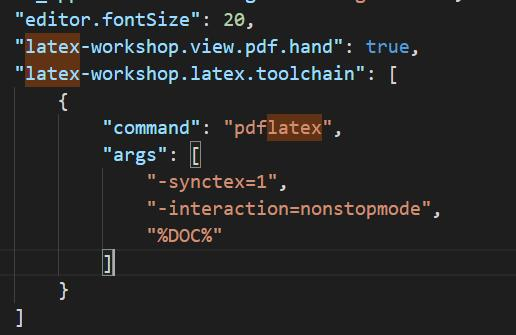
\includegraphics[width=\linewidth]{image/vscode-setting.jpg}
      \caption{设置界面.}
      \label{fig:set1}
    \end{figure}

    这是一个段落

    \paragraph{}
      这是一个段落





  \section{Latex基础}
  语法
  \begin{equation}
    f(x) = x^2
  \end{equation}

  \begin{figure}
    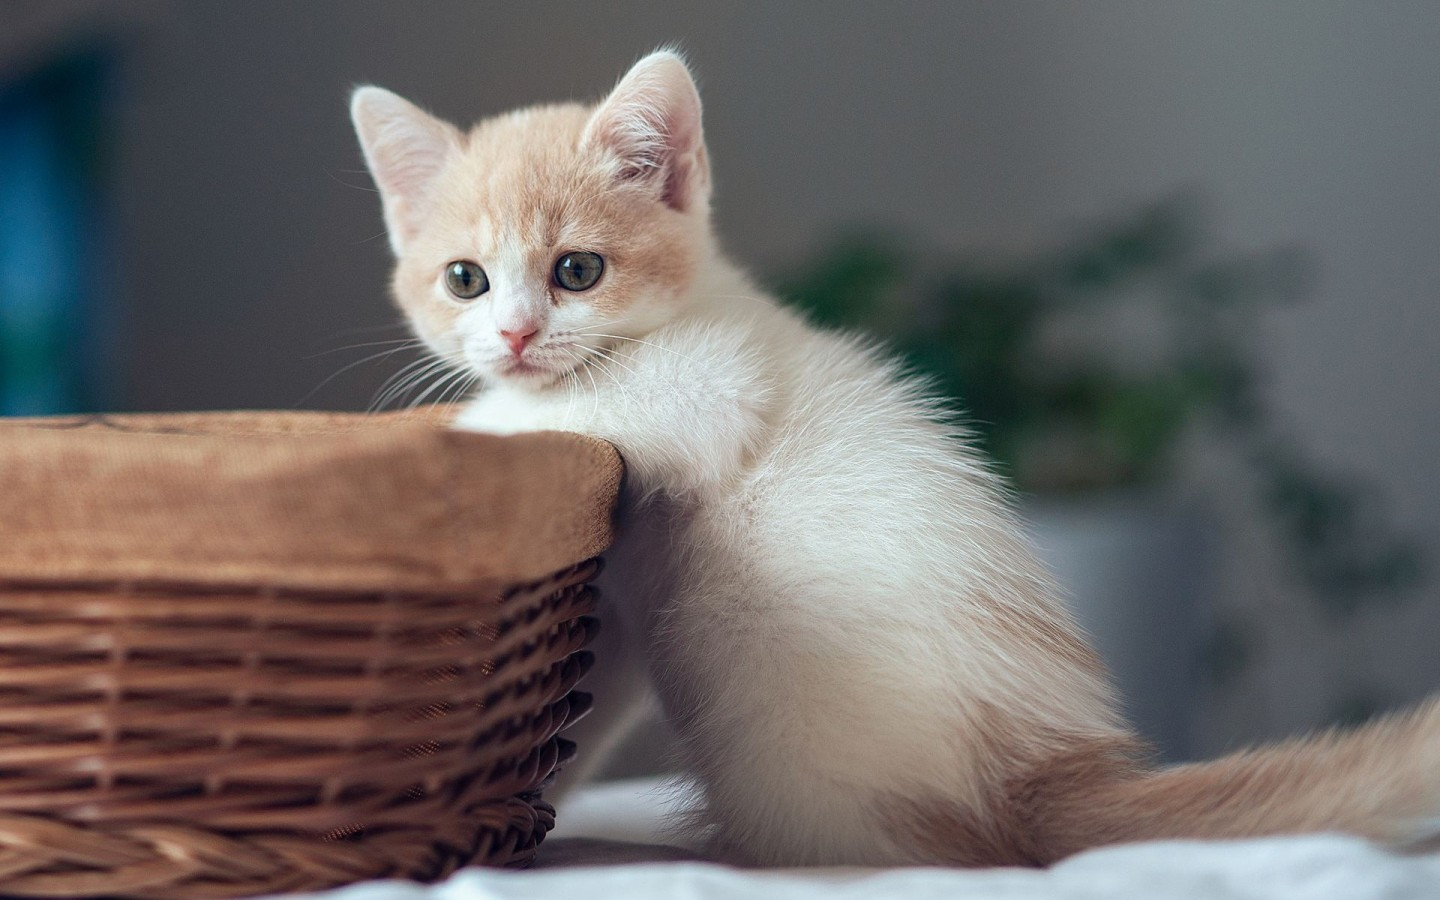
\includegraphics[width=\linewidth]{image/qwe.jpg}
    \caption{A CAT.}
    \label{fig:cat1}
  \end{figure}
  
  图 \ref{fig:cat1} shows a cat.




\end{document}
